%REPORT TEMPLATE
%AUTHOR: RUI QU  
%EMAIL: RQU@KTH.SE 

%----------------------------------------------------------------------------------------
%	PACKAGES AND DOCUMENT CONFIGURATIONS
%----------------------------------------------------------------------------------------

\documentclass{article}

%---Basic---
\usepackage{natbib} % Required to change bibliography style to APA
\usepackage{amsmath} % Required for some math elements 
\setlength\parindent{0pt} % Removes all indentation from paragraphs
\usepackage{listings}%Insert code
\usepackage{times} % Uncomment to use the Times New Roman font

%---Table---
\usepackage{multirow}%Table
\usepackage{booktabs}%Table Triple-lines
\usepackage{siunitx} % Provides the \SI{}{} and \si{} command for typesetting SI units

%---Figure---
\usepackage{graphicx} % Required for the inclusion of images
\usepackage{subfigure} % Required for multiple images
\usepackage{float} 

%---Pseudo-code in LaTeX---
\usepackage{minted} %Preference->engine->pdfTeX->Latex  ADD: -shell-escape
\usepackage{xcolor}
\definecolor{bg}{rgb}{0.95,0.95,0.95}

\usepackage{algorithm}
\usepackage{algpseudocode}
\usepackage{amsmath}
\renewcommand{\algorithmicrequire}{\textbf{Input:}}  % Use Input in the format of Algorithm
\renewcommand{\algorithmicensure}{\textbf{Output:}} % Use Output in the format of Algorithm

%---Appendix---
\usepackage{appendix}
\newcommand{\upcite}[1]{\textsuperscript{\textsuperscript{\cite{#1}}}} %Upcite

%----------------------------------------------------------------------------------------
%	DOCUMENT INFORMATION
%----------------------------------------------------------------------------------------

\begin{document}

\title{CS-E5710 Bayesian Data Analysis\\Assignment 3}                  
%\author{Rui Qu\\rui.qu@aalto.fi}
\maketitle

% If you wish to include an abstract, uncomment the lines below
% \begin{abstract}
% Abstract text
% \end{abstract}

%----------------------------------------------------------------------------------------
%	SECTION 1
%----------------------------------------------------------------------------------------

\section{Inference for normal mean and deviation}
\textbf{a)}\\
The observations follows a normal distribution, i.e. $N(\mu,\sigma^2)$ with unknown mean $\mu$ and standard deviation $\sigma$. The prior can be assumed to follow:
\begin{equation}
p(\mu,\sigma^2)=(\sigma^2)^{-1}
\end{equation}

The posterior distribution of $\mu$ follows Student's T distribution with $(n-1)$degrees of freedom, $\mu$ mean, and $\sqrt{\frac{\sigma^2}{n}}$ scale:
\begin{equation}
t_{n-1}(\mu, \sqrt{\frac{\sigma^2}{n}})=t_8(14.611, 0.491)
\end{equation}
where $n$ is the sample number, $\mu$ is the mean of observation, $\sigma$ is standard deviation.
The likelihood has the same form of posterior $t_8(14.611, 0.491)$\\
\textbf{Code:}
\begin{minted}[bgcolor=bg, linenos, fontsize=\footnotesize]{python}  
from math import sqrt
from scipy import stats
import matplotlib.pyplot as plt
import numpy as np

#data=[13.357, 14.928, 14.896, 14.820]#testdata
data=[13.357, 14.928, 14.896, 15.297, 14.82, 12.067, 
	14.824, 13.865, 17.447]
n = len(data)
mean = np.mean(data)
variance = stats.tvar(data)
interval_a=stats.t.interval(0.95,df=n-1,loc=mean,scale=sqrt(variance/n))

print('mean:',  mean)
print('variance:',  variance)
print('standard deviation:', sqrt( variance))
print('a)95% intervals:', interval_a)

x_range=np.arange(mean-3*sqrt(variance),mean+3*sqrt(variance),0.01)
y_1 = stats.t.pdf(x=x_range,df=n-1,loc=mean,scale=sqrt(variance/n))
plt.plot(x_range, y_1)
plt.savefig('./1apdf.png')
plt.title('pdf')
plt.show() 

y_2 = stats.t.cdf(x=x_range,df=n-1,loc=mean,scale=sqrt( variance/n)) 
plt.plot(x_range, y_2)
plt.savefig('./1acdf')
plt.title('cdf')
plt.show()
\end{minted}
 
\textbf{Mean:} 14.6112\\
\textbf{Variance:} 2.1731\\
\textbf{Standard deviation:} 1.4742\\
\textbf{95\% Intervals:} (13.4781, 15.7444)\\

The point estimate is 14.6112 The 95\% interval estimate can be calculated by Python function $scipy.stats.t.interval$: (13.4781, 15.7444). Then I plot pdf and cdf: \\

\textbf{Plots of probability density function and cumulative density function:}
\begin{figure}[H]
\centering  
\subfigure[pdf]{
\label{Fig.sub.1}
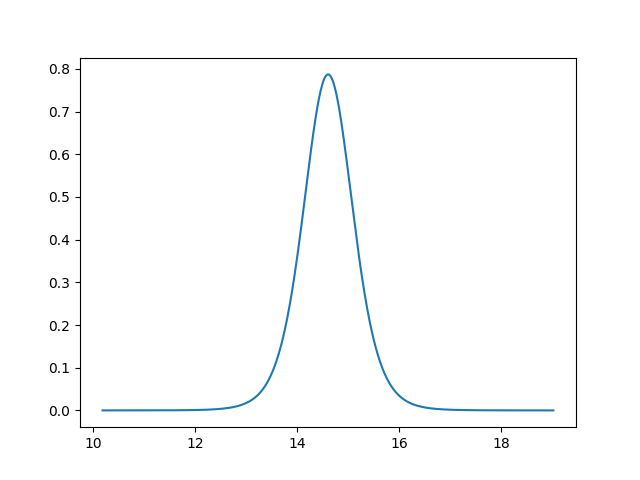
\includegraphics[width=0.485\textwidth]{1apdf.png}}
\subfigure[cdf]{
\label{Fig.sub.2}
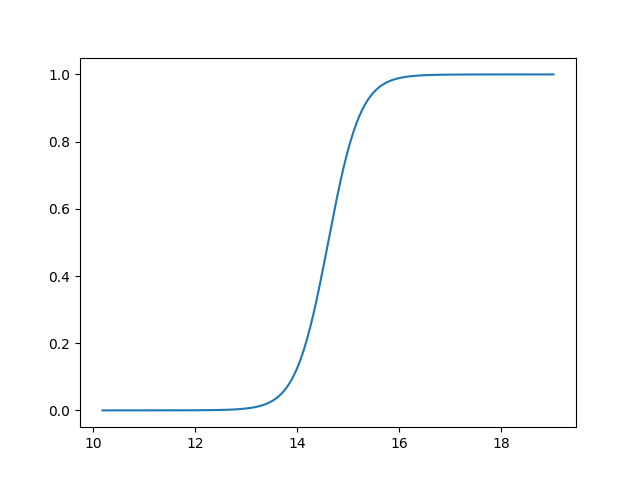
\includegraphics[width=0.485\textwidth]{1acdf.png}}
\label{Fig}
\end{figure}


\textbf{b)}\\
The posterior distribution of $\mu$ follows Student's T distribution with $(n-1)$degrees of freedom, $\mu$ mean, and $\frac{1+\frac{1}{n}}\sigma$ scale. i.e. $t_8(14.611, 1.554)$, the likelihood has the same form as posterior,$t_8(14.611, 1.554)$,
\begin{minted}[bgcolor=bg, linenos, fontsize=\footnotesize]{python}  
std_y = np.std(data, ddof=1)
scale = sqrt(1 + 1/n) * std_y
y_posterior_1= stats.t.pdf(x=x_range,df=n-1,loc= mean, scale=scale)

y_posterior_2=stats.t.cdf(x=x_range,df=n-1,loc= mean,scale=scale)
interval_b = stats.t.interval(0.95,df=n-1,loc=mean, scale=scale)
print('b) 95%interval',interval_b)

figure = plt.plot(x_range, y_posterior_1)
plt.savefig('./1bpdf.png')
plt.title('pdf')
plt.show()

figure = plt.plot(x_range, y_posterior_2)
plt.savefig('./1bcdf.png')
plt.title('cdf')
plt.show()
\end{minted}
\textbf{95\%interval:} (11.0279, 18.1945)\\

The posterior mean is equal to the observation mean. The expected value of the point estimate is \textbf{14.6112} The 95\% interval can be calculated by Python function $scipy.stats.t.interval()$: \textbf{(11.0279, 18.1945)}. Then I plot pdf and cdf: \\

\textbf{Plots of density functions:}
\begin{figure}[H]
\centering  
\subfigure[pdf]{
\label{Fig.sub.1}
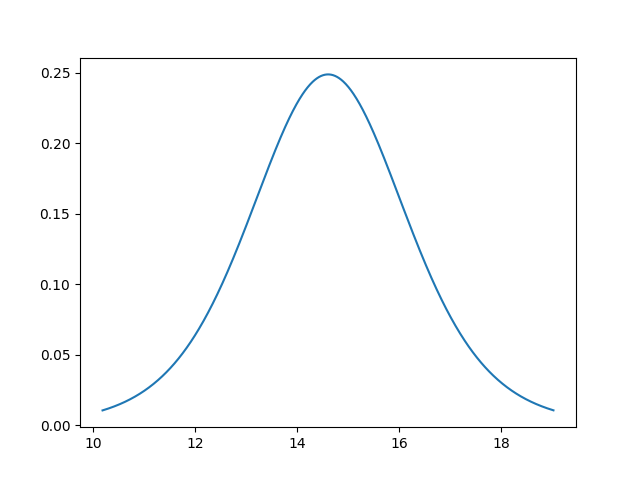
\includegraphics[width=0.485\textwidth]{1bpdf.png}}
\subfigure[cdf]{
\label{Fig.sub.2}
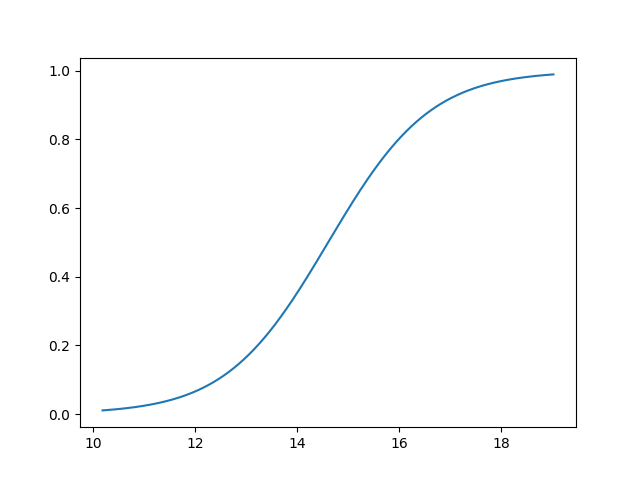
\includegraphics[width=0.485\textwidth]{1bcdf.png}}
\label{Fig}
\end{figure}

\section{Inference for the difference between proportions}
\textbf{a)}\\

The noninformative prior can take the Jeffery's prior model. i.e. $p(p_0)=p(_1)=Beta(\frac{1}{2},\frac{1}{2})$ The resulting posterior is given as following:
\begin{equation}
\begin{aligned}
&Beta(0.5+x,0.5+x-y)\\
&p_0=Beta(0.5+39, 0.5+674-39)=Beta(39.5, 635.5)\\
&p_1=Beta(0.5+22, 0.5+680-22)=Beta(22.5, 658.5)
\end{aligned}
\end{equation}
where x is the number of observations, y is the number of mortality observation in this case. The likelihood has the same form of posterior.\\

\textbf{Code:}
\begin{minted}[bgcolor=bg, linenos, fontsize=\footnotesize ]{python}  
from scipy import stats
import matplotlib.pyplot as plt
import numpy as np

x_range = np.arange(0, 0.2, 0.001)
control = 674
control_died = 39
control_a = control_died + .5
control_b = control - control_a + .5
control_posterior = control_a/control
control_pdf = stats.beta.pdf(x_range, control_a, control_b)

treatment = 680
treatment_died = 22
treatment_a = treatment_died + .5
treatment_b = treatment - treatment_a + .5
treatment_posterior = treatment_a/treatment

control_pdf = stats.beta.pdf(x_range, control_a, control_b)
treatment_pdf = stats.beta.pdf(x_range, treatment_a, treatment_b)
plt.plot(x_range, control_pdf,label='Control group')
plt.plot(x_range, treatment_pdf,label='Treatment group')
plt.legend()
plt.savefig('./2apdf.png')
plt.show()

control_cdf = stats.beta.cdf(x_range, control_a, control_b)
treatment_cdf = stats.beta.cdf(x_range, treatment_a, treatment_b)
plt.plot(x_range, control_cdf,label='Control group')
plt.plot(x_range, treatment_cdf,label='Treatment group')
plt.legend()
plt.savefig('./2acdf.png')
plt.show()

p_control = stats.beta.rvs(control_a, control_b, size=100000)
p_treatment = stats.beta.rvs(treatment_a, treatment_b, size=100000)
odd_ratio = (p_treatment/(1-p_treatment))/(p_control/(1-p_control))

plt.hist(odd_ratio, alpha=0.5, bins=40, ec='white',color='grey')
plt.savefig('./2ahist.png')
plt.show()

mean = np.mean(odd_ratio)
print('mean',mean)
print('95% Intervals', (np.percentile(odd_ratio, 2.5), 
	np.percentile(odd_ratio, 97.5)))
print('90% Intervals', (np.percentile(odd_ratio, 5), 
	np.percentile(odd_ratio, 95)))
\end{minted}

\textbf{mean:}0.5643\\
\textbf{95\% Intervals:} (0.3163, 0.9191)\\
\textbf{90\% Intervals:} (0.3459, 0.8453)\\

To briefly introduce the code, I randomly sample from 2 groups of the distribution by Python function $scipy.stats.beta.rvs(a,b,size=100000)$ and calculate ratio by the given formula in instruction. The expected value of posterior distribution can be calculated by $np.mean(odd_ratio)$,which is 0.5643 The 95\% interval is (0.3163, 0.9191). Then I plot pdf, cdf of 2 groups respectively as well as the histgram.\\

\textbf{Plots of density functions:}
\begin{figure}[H]
\centering  
\subfigure[pdf]{
\label{Fig.sub.1}
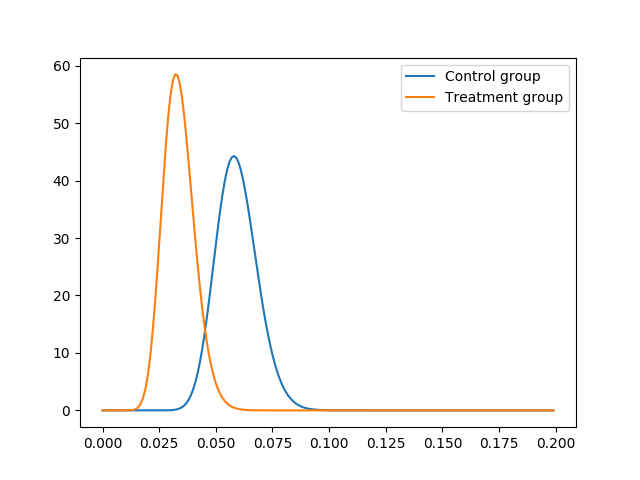
\includegraphics[width=0.485\textwidth]{2apdf.png}}
\subfigure[cdf]{
\label{Fig.sub.2}
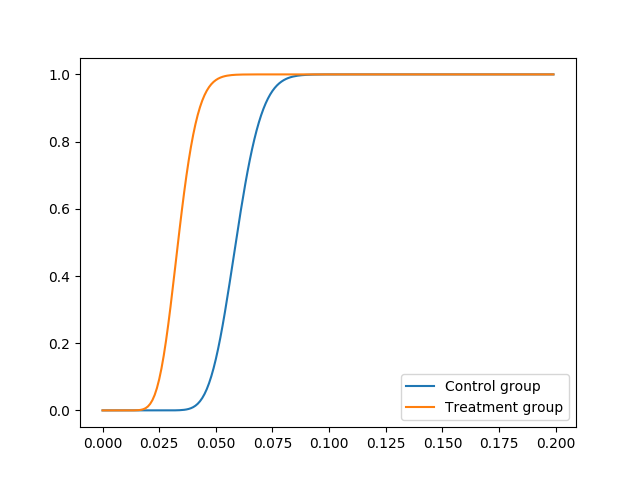
\includegraphics[width=0.485\textwidth]{2acdf.png}}
\label{Fig}
\end{figure}

\textbf{Plot of histgram:}
\begin{figure}[H]
\centering  
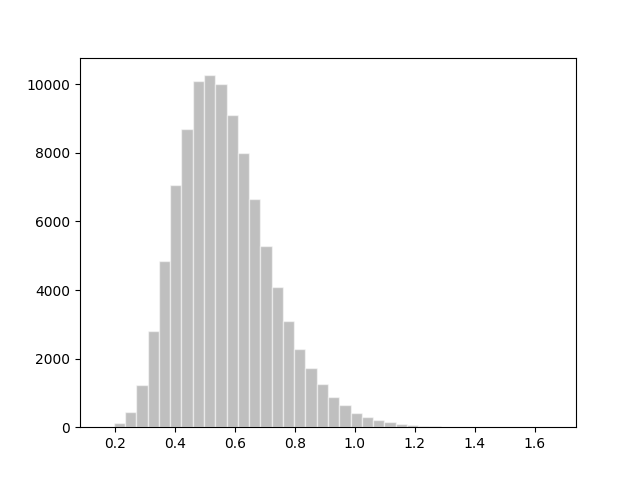
\includegraphics[scale=0.5]{2ahist.png}
\label{Fig}
\end{figure}

\textbf{b)}\\
To test difference between different prior densities, I change the prior in my code to $Beta(1,1)$ and got estimated posterior is 0.5700 and 95\% interval is (0.3216, 0.9257) which are  quite similar to those of $Beta(\frac{1}{2},\frac{1}{2})$. The difference between priors from $Beta(0,0)$ to $Beta(1,1)$ comes down to a single dead or undead for the posterior distribution in this case. Thus, the results of them are quite close. We could say that the posterior density is not sensitive to the choice of prior density.  \\




\section{Inference for the difference between normal means}
\textbf{a)}\\
In this case for both two datasets, the prior follows $p(\mu, \sigma^2)=\frac{1}{\sigma^2}$, the resulting posterior follows Student's T distribution $t_{n-1}(\mu,\frac{\sigma^2}{n})$, the likelihood has the same form as posterior $t_{n-1}(\mu,\frac{\sigma^2}{n})$ \\

\textbf{Code:}
\begin{minted}[bgcolor=bg, linenos, fontsize=\footnotesize]{python}  
from math import sqrt
import scipy
from scipy import stats
import matplotlib.pyplot as plt
import numpy as np

def model(data):
    n = len(data)
    mean = np.mean(data)
    variance = stats.tvar(data)
    x_range = np.arange(
        mean - 3 * sqrt(variance),
        mean + 3 * sqrt(variance),
        0.01)
    mu = stats.t.pdf(x=x_range,df=n-1,loc=mean,scale=sqrt(variance/n))
    return n, mean, variance, x_range, mu

data_1 = [13.357,14.928,14.896,15.297,14.82,12.067,14.824,13.865,17.447]
data_2 = [15.98,14.206,16.011,17.25,15.993,15.722,17.143,15.23,15.125,
	16.609,14.735,15.881,15.789]
n_1, mean_1, variance_1, x_range_1, mu_1 = model(data_1)
n_2, mean_2, variance_2, x_range_2, mu_2 = model(data_2)

mu_1=stats.t.rvs(df=n_1-1,loc=mean_1,scale=sqrt(variance_1/n_1),
	size=100000)
mu_2=stats.t.rvs(df=n_2-1,loc=mean_2,scale=sqrt(variance_2/n_2),
	size=100000)
mu_d=mu_1 - mu_2

plt.hist(mu_d, bins=50, ec='white', color='grey', alpha=0.5)
plt.savefig('./3.png')
plt.show()

interval_1=stats.t.interval(0.95,df=n_1-1,loc=mean_1,
	scale=sqrt(variance_1/n_1))
interval_2=stats.t.interval(0.95,df=n_2-1,loc=mean_2,
	scale=sqrt(variance_2/n_2))

print('windshieldy1 mean',model(data_1)[1])
print('windshieldy2 mean',model(data_2)[1])
print('windshieldy1 95% interval',interval_1)
print('windshieldy2 95% interval',interval_2)

print('mean diff 95% Intervals', np.mean(mu_d))
print('mean diff 95% Intervals',np.percentile(mu_d, 2.5),np.percentile(mu_d,97.5)
print('Percentile of mu less than 0 'stats.percentileofscore(mu_d, 0), '%')
\end{minted}

\textbf{Windshieldy1 mean} 14.6112\\
\textbf{Windshieldy2 mean} 15.8211\\
\textbf{Windshieldy1 95\% interval} (13.4781, 15.7444)\\
\textbf{Windshieldy2 95\% interval} (15.2938, 16.3484)\\
\textbf{Mean's difference mean} -1.2082\\
\textbf{Mean's difference 95\% Intervals} (-1.782, -0.6406)\\
\textbf{Percentile of mu less than 0} 97.304 \%\\

The calculation of estimated posterior and 95\% intervals is similar to the exercise 1. Point estimate for the means' difference is \textbf{-1.2082} and interval estimates (95\%) is \textbf{(-1.782, -0.6406)}  \\

\textbf{Plot of histgram:}
\begin{figure}[H]
\centering  
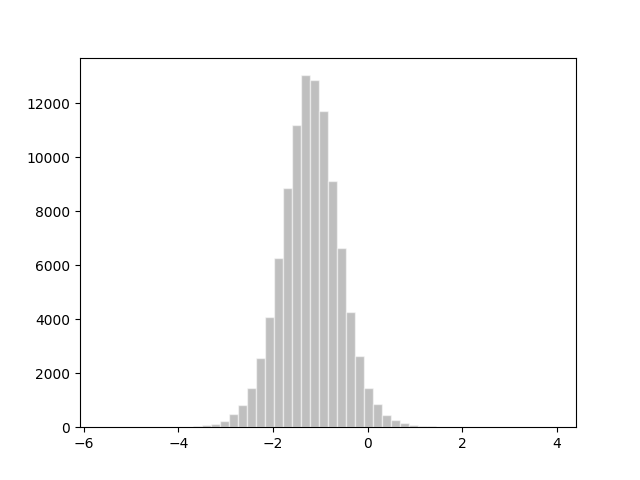
\includegraphics[scale=0.5]{3.png}
\label{Fig}
\end{figure}

\textbf{b)}\\
The means are not the same. Firstly, the means of two distribution are different. Secondly the percentile of $\mu<0$ is 97.304 \% we can conclude that they're not the same.




\end{document}